\documentclass{beamer} % [aspectratio=169]
\usetheme{ucl}
\setbeamercolor{banner}{bg=darkred}
\setbeamersize{description width=2em}
\setbeamertemplate{navigation symbols}{\vspace{-2ex}} 
\usepackage{soul}

%\usepackage{fontspec}
\usepackage[utf8]{inputenc}

\usepackage[T1]{fontenc} % Turn £ into $
\usepackage{minted}
\usemintedstyle{emacs}

\usepackage{fancyvrb}
\usepackage{xcolor}
\usepackage{url}

\usepackage{natbib}
\usepackage{bibentry}
\usepackage{url}


\usepackage{tikz}
\usetikzlibrary{positioning}
\usetikzlibrary{calc,shapes.multipart,chains,arrows}
\usetikzlibrary{shapes,snakes}

\tikzset{
  treenode/.style = {align=center, inner sep=0pt, text centered,
    font=\sffamily},
  arn_n/.style = {treenode, circle, draw=black,
     text width=1.5em},% arbre rouge noir, noeud noir
  arn_r/.style = {treenode, circle, red, draw=red, 
    text width=1.5em, very thick},% arbre rouge noir, noeud rouge
  arn_d/.style = {treenode, star, star points=10, red, draw=red, 
    text width=1.5em, very thick},% arbre rouge noir, noeud rouge
  arn_x/.style = {treenode, rectangle, draw=black}% arbre rouge noir, nil
}

\newcommand\emc[1]{\textcolor{midred}{\textbf{#1}}}

\AtBeginSection[]{
  \begin{frame}
  \vfill
  \centering
  \begin{beamercolorbox}[sep=8pt,center,shadow=true,rounded=true]{title}
    \usebeamerfont{title}\insertsectionhead\par%
  \end{beamercolorbox}
  \vfill
  \end{frame}
}

\author{Mark Handley\\
  {\small based on slides by George Danezis}}
\title{Develpment Practices, Modules, Tools \& Releases.}
\subtitle{ENGF0002: Design and Professional Skills }
% \institute{}
\date{Term 1, 2019}


\begin{document}
\nobibliography*


\frame{
\titlepage
}

\section{Python packages, libraries, and deployment.}


\begin{frame}

\frametitle{Import Python libraries}


Import a library by name:
  \inputminted[
    firstline=3,
    lastline=5,
    xleftmargin=1.4em,
    frame=lines,
    framesep=2mm,
    %baselinestretch=1.2,
    % bgcolor=lightgray,
    fontsize=\scriptsize,
    linenos
  ]{python}{src/example_import.py}

Import specific names within the library:
  \inputminted[
    firstline=7,
    lastline=8,
    xleftmargin=1.4em,
    frame=lines,
    framesep=2mm,
    %baselinestretch=1.2,
    % bgcolor=lightgray,
    fontsize=\scriptsize,
    linenos
  ]{python}{src/example_import.py}

Import and rename a library:
  \inputminted[
    firstline=11,
    lastline=12,
    xleftmargin=1.4em,
    frame=lines,
    framesep=2mm,
    %baselinestretch=1.2,
    % bgcolor=lightgray,
    fontsize=\scriptsize,
    linenos
  ]{python}{src/example_import.py}

Look for library in the folders \texttt{sys.path}.

\end{frame}

\begin{frame}

\frametitle{The Python Standard Library}

The standard libraries are available with any full python installation. You can \emc{rely on them}!
\begin{itemize}
  \item \emc{Basic programming}: Built-in types, text processing, binary data, dates, calendars, maths, functional tools, \ldots
  \item \emc{System}: Files, directories, data formats, compression, cryptography, operating system functions, \ldots
  \item \emc{Communications}: Inter-process communications, internet protocols, markup, multimedia, i19n, \ldots
  \item \emc{Language}: Debug / profile, distrbute, runtime, interpreters, import, language, \ldots
  \end{itemize}

Always \emc{prefer to use the standard library} over your own types.

\end{frame}

\begin{frame}

\frametitle{Non-standard libraries}

Third party libraries require \emc{additional installation}. \emc{Useful ones}:

\begin{description}
  \item[numpy,scipy] Numeric \& scientific libraries and linear algebra.
  \item[matplotlib] Scientific graphs and plots.
  \item[pandas] Manipulation of tabular data.
  \item[OpenCV,scikit-learn,Pytorch,Theano,TensorFlow] Machine learning.
  \item[tox, pytest, sphinx] Tests, documentation.
  \item[requests,django,flask] Web requests and web app servers.
  \item[fabric,doit] DevOps.
  \item[cffi\hspace{0.5in}] \hspace{-0.5in}Bind to low-level C code.  %work around beamer bug
\end{description}
\end{frame}


\begin{frame}

\frametitle{Should you take a dependency?}

Issues to consider before relying on a 3rd party library:
\begin{itemize}
\item \emc{Quality}: is it going to be any good? Good Documentation; No Bugs.
\item \emc{Community}: is it being used by many? is it being maintained? Release schedule, responsiveness to bug reports, and breaking downstreams.
\item \emc{Trust}: do you believe maintainers will attack your software?
\item \emc{License}? are you allowed to use it?
\end{itemize}

\begin{block}{}
If you are the biggest user of a library by far, you may end up having to also be the maintainer.
\end{block}

\end{frame}

\begin{frame}

\frametitle{Understanding Intellectual Property}

The state is protecting creators to incentivise investment in new inventions.
\begin{itemize}
  \item \emc{Copyright}: protects authors of artistic or literary works, including software! if you write something you (or employer) own the copyright -- can transfer it, or license it.
  \item \emc{Trade marks}: protect your trading image, name, logos, etc. to avoid brand and consumer confusion. You might have to register them.
  \item \emc{Patents}: apply and get issued one for an invention. Disclose the invention, but get protection for a limited time. Status of software patents is problematic.
\end{itemize}

\end{frame}

\begin{frame}

\frametitle{Licensing your own software, or using licensed software.}

A software license is an agreement between a creator and a user of a work, about the conditions under which the user may use the creations. 

\begin{itemize}
  \item \emc{Commercial}: creator gets some money, and in return allows use of software. Usually no other rights are transfered.
  \item \emc{Free Software}: creator allows user all rights, including modifying software. But does not allow endorsement, or liability. May or not grant \emc{rights to patents}. \\
  eg.\ BSD, MIT, Apache.
  \item \emc{Gnu Public Licenses}: like free software, but \emc{viral}. Requires any modifications to also become free software under the same license. \\ eg.\ GPLv2, GPLv3, LGPL.
\end{itemize}

\emc{Check license} before using libraries!

\end{frame}

\begin{frame}
  %\frametitle{BSD License.}
  \hspace{-8mm}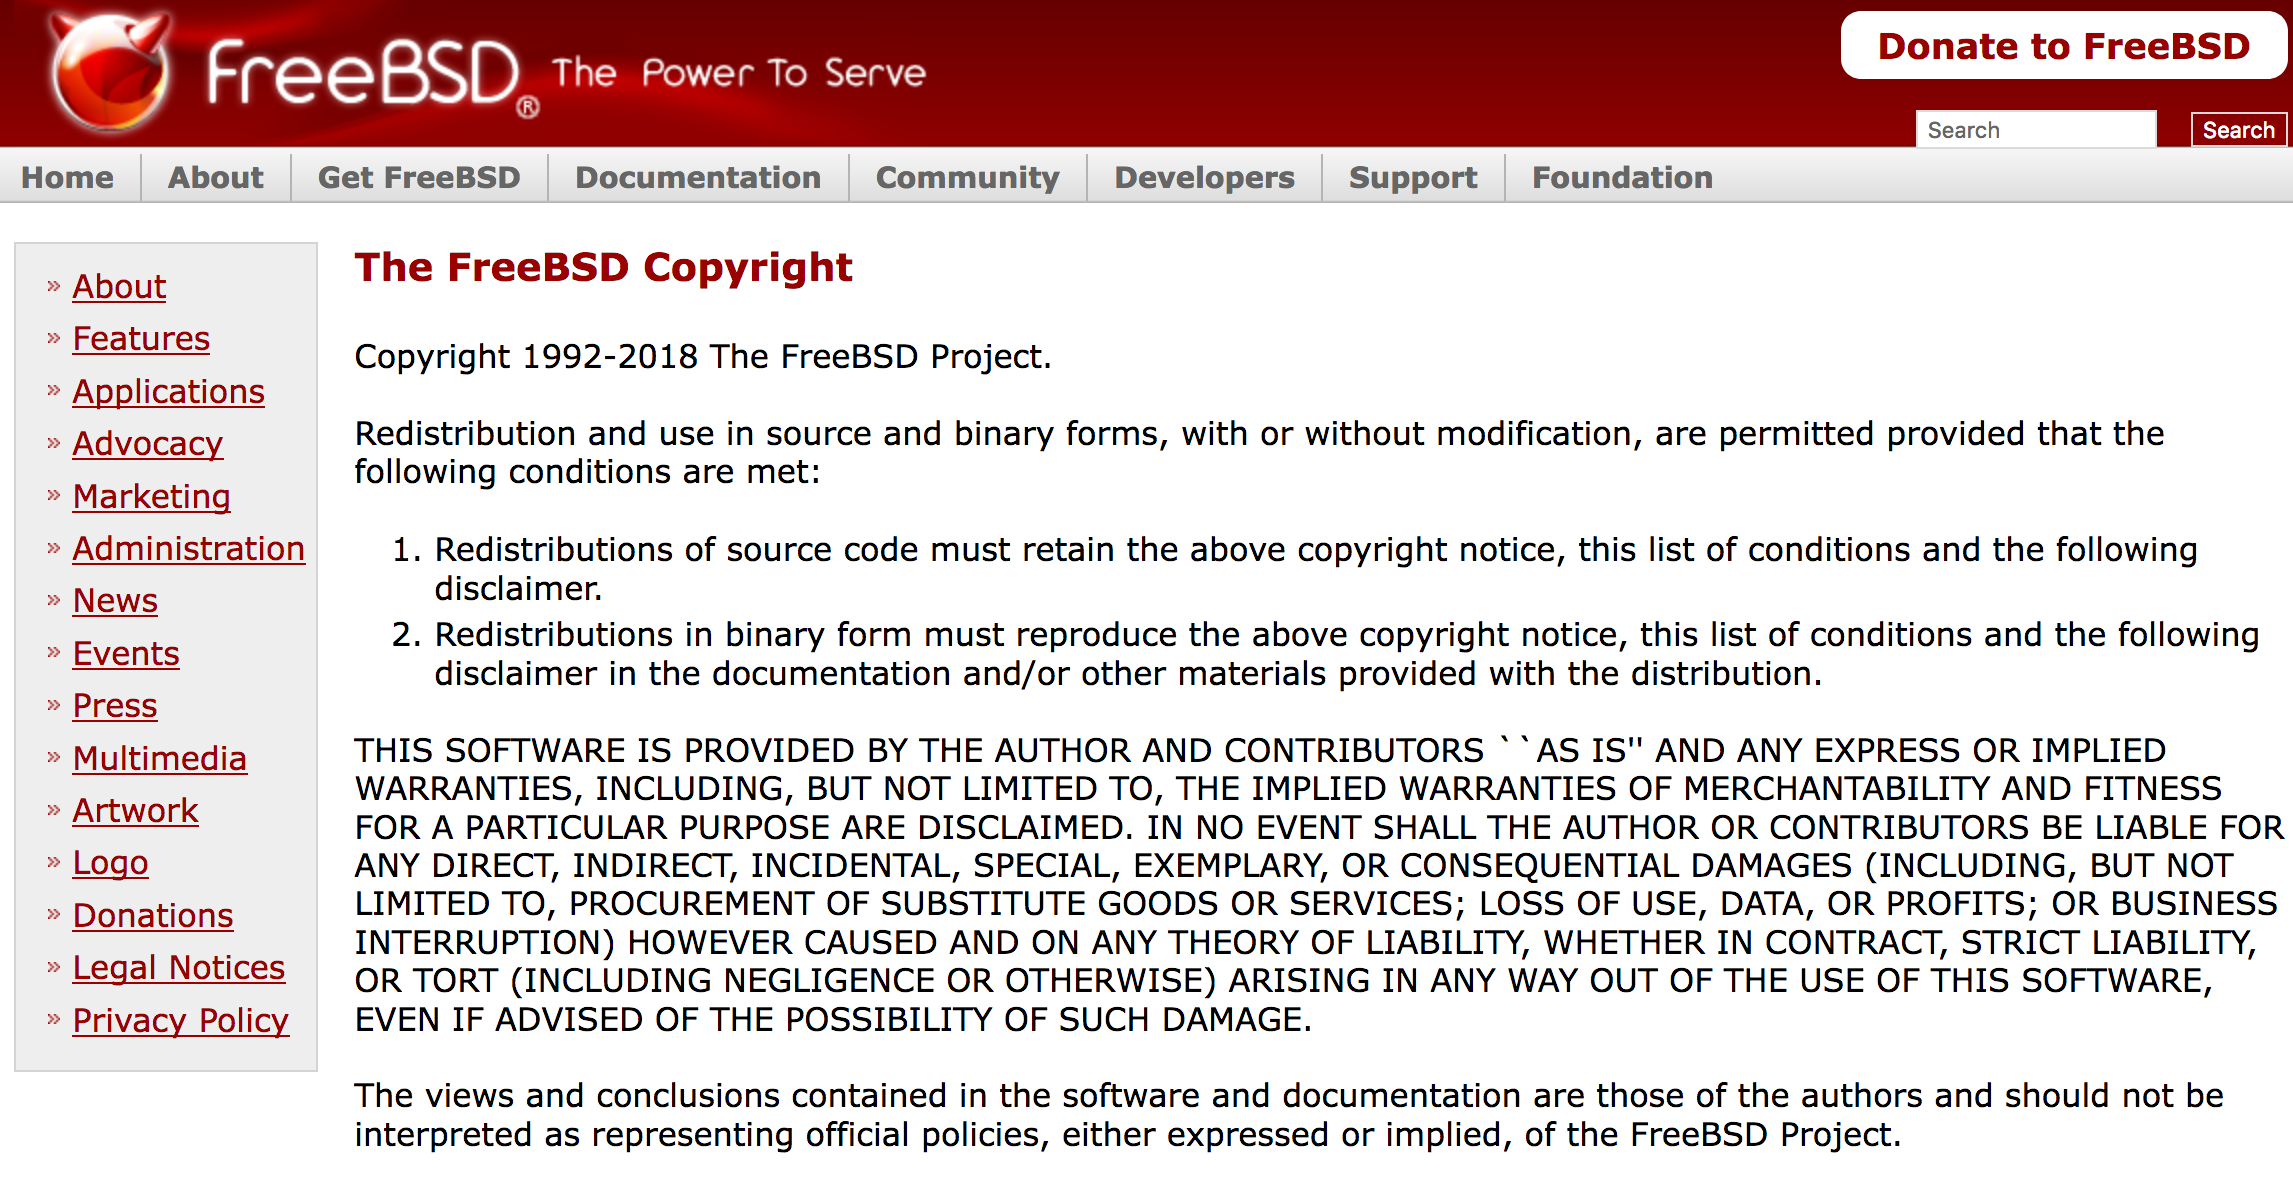
\includegraphics[height=65mm]{assets/freebsd}
\end{frame}

\begin{frame}
  %\frametitle{GPL License.}
  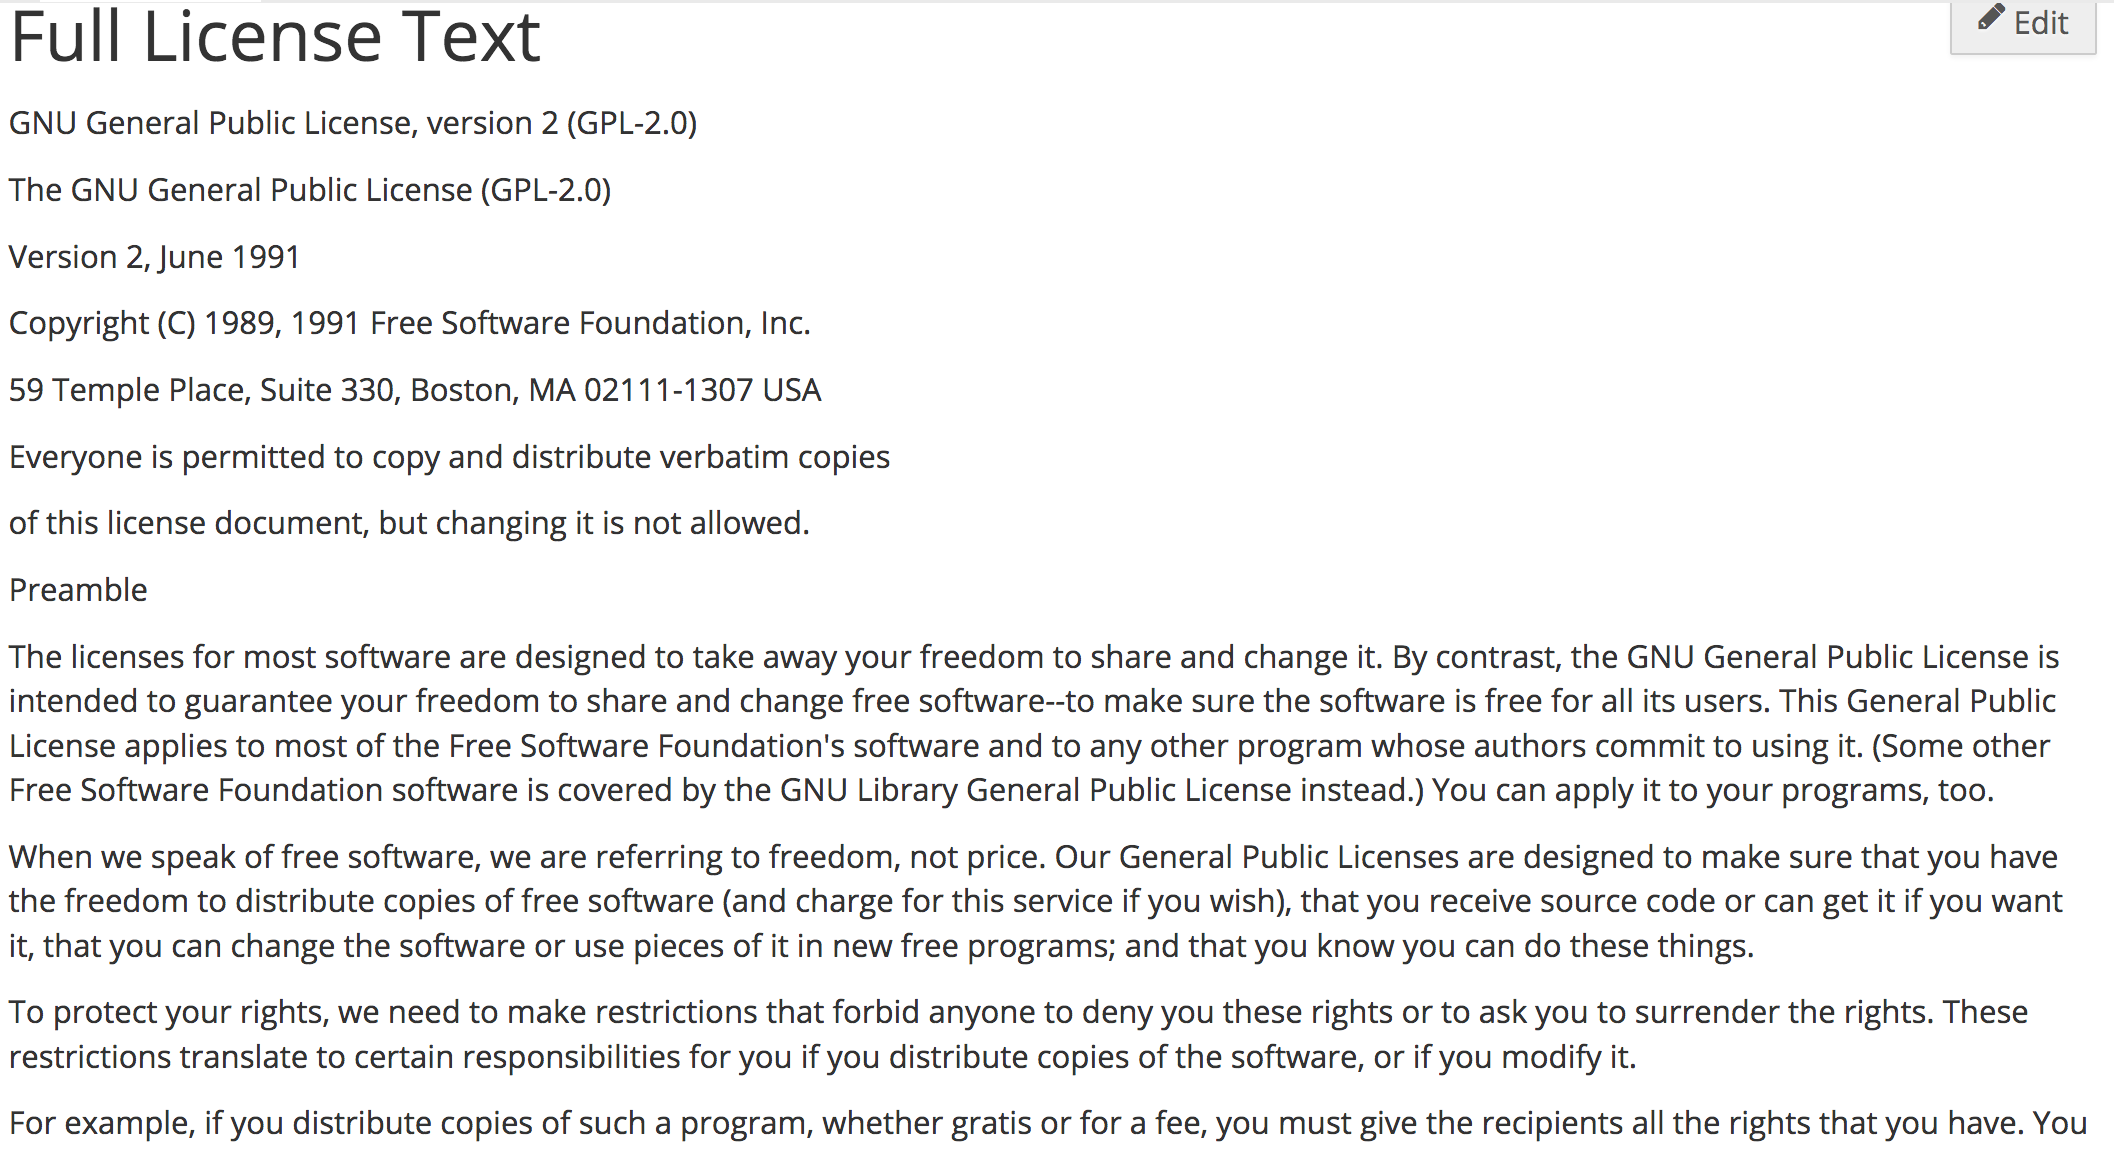
\includegraphics[height=65mm]{assets/gplv2}
\end{frame}

\begin{frame}

\frametitle{Philosophical discussion: what is more `free'?}

Question 1. Viral licenses impose more restrictions on users, but guarantee the resulting software is also free. Are they more or less in line with ideas of software freedom?

\vspace{5mm}

Question 2. Discuss the statement `A good non-viral library will inevitably end up being extended commercially and become closed source / non-free as a result.'

\vspace{5mm}

Question 3. What incentives are there for commercial entities to contribute to free software?

\vspace{5mm}
Also, study controversies around software patents: \url{http://endsoftpatents.org/}

\end{frame}

\begin{frame}[fragile]

\frametitle{Installing 3rd party modules}

List of great Python modules: \url{https://github.com/vinta/awesome-python}

Python Package repository, \emc{Pypi}: \url{https://pypi.python.org/pypi}

\vspace{3mm}
Python comes with \texttt{pip} as a package manager:
\begin{verbatim}
$ pip install <modulename>
\end{verbatim}
Full \texttt{pip} documentation: \url{https://pip.pypa.io/en/stable/}

\end{frame}


\begin{frame}[fragile]

\frametitle{Clashing versions of modules}

What to do if you need two different (clashing) versions of the same library?

What about testing your program or library using different library versions?

\vspace{5mm}
Solution: use \texttt{virtualenv} to create a clean virtual environment:
\begin{small}
\begin{verbatim}
$ virtualenv ENV           # Create in dir ENV
$ source ENV/bin/activate  # Activate environment
(ENV)$ pip install ...     # Install in ENV
(ENV)$ python ...          # Run in ENV
(ENV)$ deactivate          # Exit ENV
$
\end{verbatim}
\end{small}

\end{frame}


\begin{frame}

\frametitle{Make your own libraries and modules}

Why think of programs in terms of modules?
\begin{itemize}
  \item Most programs are too big to live in a single file.
  \item Clean, well defined interfaces between modules, reduce communication overheads. 
  \item Information Hiding behind modules allows for abstraction and maintainability.
  \item Controlled interactions allow decoupling of modules.
  \item High-quality, reusable code -- can be used across projects.
\end{itemize}

\end{frame}

\begin{frame}[fragile]

\frametitle{Lightweight libraries and modules}

Python allows a program to be \emc{split across many files}. 

\vspace{3mm}
Consider the two files:
\begin{verbatim}
branch.py
minimap.py
\end{verbatim}

\vspace{3mm}
Each creates a \emc{name space available to the other} through \texttt{import}. \\ Eg. in \texttt{minimap.py}:
\begin{minted}{python}
from branch import branch
\end{minted}

\end{frame}

\begin{frame}

\frametitle{From many files, to libraries, to modules \ldots}

\end{frame}


\begin{frame}[fragile]

\frametitle{The structure of a module}

All user-facing libraries, and Python end-user programs are usually packaged as \emc{modules}.

\vspace{3mm}
Module \texttt{<mymodule>} is a directory of files:
\begin{small}
\begin{Verbatim}[fontsize=\footnotesize]
README.rst                # Basic help on github
LICENSE                   # License
setup.py                  # Packaging & dependencies information
tox.ini                   # Test setup
euclid/__init__.py        # Modules code
euclid/gcd.py
docs/conf.py              # Module Sphinx documentation
docs/index.rst
tests/test_gcd.py         # Module tests
\end{Verbatim}
\end{small}

See The Hitchhiker’s Guide to Python \url{http://docs.python-guide.org/en/latest/}

\end{frame}


\begin{frame}

\frametitle{The GCD function -- as before}  


We define our GCD function in \texttt{euclid/gcd.py}
  \inputminted[
    xleftmargin=1.4em,
    %frame=lines,
    %framesep=2mm,
    %baselinestretch=1.2,
    bgcolor=stone,
    fontsize=\scriptsize,
    %linenos
  ]{python}{src/euclid/euclid/gcd.py}


\end{frame}

\begin{frame}

\frametitle{The module \texttt{\_\_init\_\_.py} file}

A \texttt{euclid/\_\_init\_\_.py} file indicates the directory defines a module.

\vspace{5mm}
The code in the file defines names within the module.

\vspace{5mm}
The variable \texttt{\_\_all\_\_} restricts the names exported, \\ by eg. \texttt{from euclid import *}.
\end{frame}

\begin{frame}

\frametitle{The module \texttt{\_\_init\_\_.py} file}
  
  \inputminted[
    xleftmargin=1.4em,
    %frame=lines,
    %framesep=2mm,
    %baselinestretch=1.2,
    bgcolor=stone,
    fontsize=\scriptsize,
    %linenos
  ]{python}{src/euclid/euclid/__init__.py}

\end{frame}

\begin{frame}

\frametitle{The module \texttt{setup.py}}

  \inputminted[
    xleftmargin=1.4em,
    %frame=lines,
    %framesep=2mm,
    %baselinestretch=1.2,
    bgcolor=stone,
    fontsize=\scriptsize,
    %linenos
  ]{python}{src/euclid/setup.py}

\end{frame}

\begin{frame}

\frametitle{The \texttt{setup.py} meta-data}

\begin{itemize}
  \item The \emc{name} and \emc{version} are used by pip / pypi to index your package.
  \item The \emc{packages} point to what is included in the module. \\ (Note that tests are not included in this case.)
  \item The \emc{install\_requires} lists packages required. \\ Can specify \emc{version range}. 
  \item The \emc{entry\_points} list the function that starts an application.
  \end{itemize}

\end{frame}

\begin{frame}[fragile]

\frametitle{Packaging the module}

Create a \emc{source distribution} using:
\begin{verbatim}
$ python setup.py sdist
\end{verbatim}

\vspace{3mm}
Create a \emc{binary distribution} using:
\begin{verbatim}
$ python setup.py bdist
$ python setup.py bdist --format=wininst
\end{verbatim}

\vspace{3mm}
\emc{Install manually} a package:
\begin{verbatim}
$ python setup.py install
\end{verbatim}

\end{frame}

\begin{frame}

\frametitle{Testing packaging and installation using \texttt{tox}}

\begin{itemize}
  \item Need to test packaging.
  \item Need to test install process.
  \item Need to test against many Python versions.
  \item Need to test against many library versions.
  \end{itemize}

  \vspace{5mm}
  The tool of choice for this is \texttt{tox}. You can define \emc{environments}, \emc{dependencies}, and \emc{commands} to test in them

\end{frame}


\begin{frame}
  \frametitle{Tox workflow}
  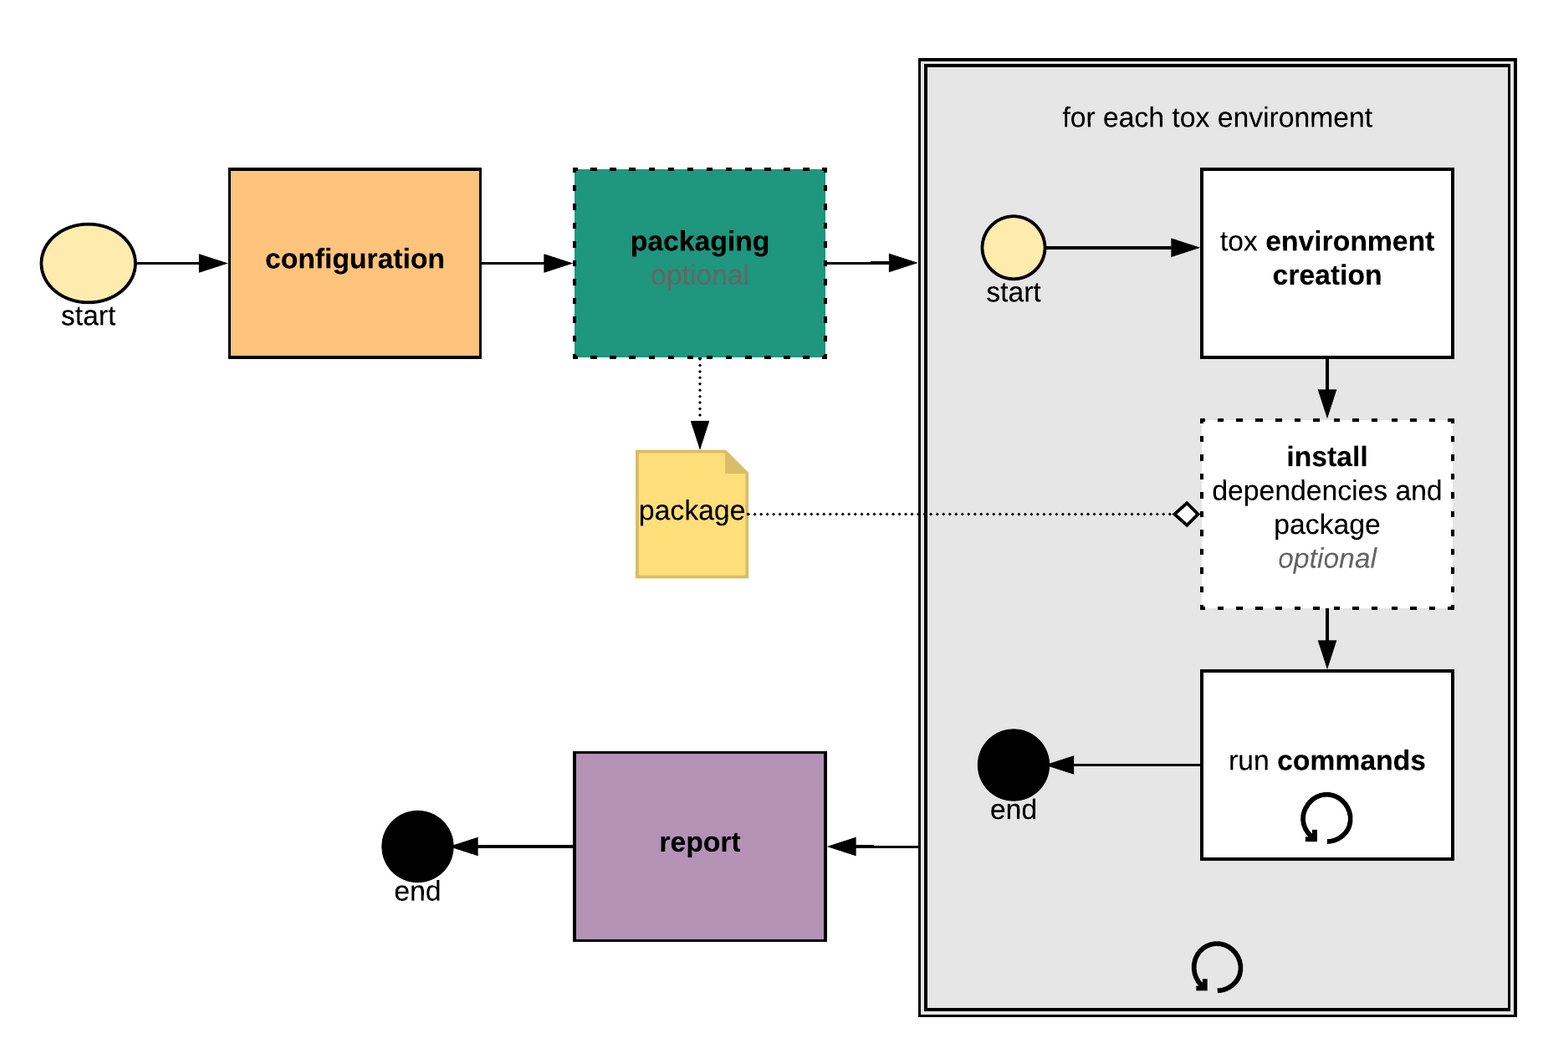
\includegraphics[height=65mm]{assets/tox}
\end{frame}


\begin{frame}[fragile]

\frametitle{The \texttt{tox.ini} file}

Test in a Python 3.5 context \ldots 
\begin{scriptsize}
\begin{verbatim}
[tox]
envlist = py35

[testenv]
deps = pytest
       pytest-cov

commands = pytest --doctest-modules -sv euclid
           pytest --cov={envsitepackagesdir}/euclid --doctest-modules -sv tests
           euclid 10 2
\end{verbatim}
\end{scriptsize}
\ldots and execute pytest, coverage and the program itself.

\end{frame}


\begin{frame}[fragile]
\begin{tiny}
\begin{verbatim}
$ tox
GLOB sdist-make: src\euclid\setup.py
py35 inst-nodeps: src\euclid\.tox\dist\euclid-0.0.1.zip
py35 installed: coverage==4.4.2, euclid==0.0.1, pytest==3.3.0, pytest-cov==2.5.1
py35 runtests: commands[0] | pytest --doctest-modules -sv euclid
============================= test session starts =============================
collecting ... collected 1 item

euclid/gcd.py::euclid.gcd.GCD PASSED                                     [100%]
========================== 1 passed in 0.03 seconds ===========================
py35 runtests: commands[1] | pytest --cov=site-packages/euclid --doctest-modules -sv tests
============================= test session starts =============================
collecting ... collected 5 items

tests/test_gcd.py::test_euclid PASSED                                    [ 20%]
tests/test_gcd.py::test_euclid_exc PASSED                                [ 40%]
tests/test_gcd.py::test_euclid_exc_raises[test_inputs0] PASSED           [ 60%]
tests/test_gcd.py::test_euclid_exc_raises[test_inputs1] PASSED           [ 80%]
tests/test_gcd.py::test_euclid_exc_raises[test_inputs2] PASSED           [100%]
----------- coverage: platform win32, python 3.5.3-final-0 -----------
Name                                             Stmts   Miss  Cover
--------------------------------------------------------------------
.tox\py35\Lib\site-packages\euclid\__init__.py      16     11    31%
.tox\py35\Lib\site-packages\euclid\gcd.py            6      0   100%
--------------------------------------------------------------------
TOTAL                                               22     11    50%
========================== 5 passed in 0.06 seconds ===========================
py35 runtests: commands[2] | euclid 10 2
2
___________________________________ summary ___________________________________
  py35: commands succeeded
  congratulations :)
\end{verbatim}
\end{tiny}

\end{frame}

\begin{frame}

\frametitle{Documentation}

Use \emc{Sphinx} and \emc{autodoc} to generate documentation. 
\begin{itemize}
  \item Include (and test) examples in your documentation!
  \item Test your examples! (\texttt{pytest --doctest-modules -sv euclid})
  \item Provide testing documentation -- so that others can hack on your code.
\end{itemize}

\vspace{3mm}
Execute \texttt{sphinx-quickstart} to start your Sphinx documentation.
\end{frame}


\begin{frame}[fragile]

\frametitle{Documentation with \texttt{autodoc}}

Write \texttt{index.rst}. Compile with \texttt{docs/make html}:
\begin{tiny}
\begin{verbatim}
Welcome to euclid's documentation!
==================================

The euclid module provides an implementation of the Greatest Common Denominator (GCD) algorithm. 
It provides a command line utility to compute the GCD::

    $ euclid 10 2
    2

The Euclid Python module
------------------------

.. autofunction:: euclid.GCD

Development
-----------

To test the Euclid module, use tox::

    $ tox

\end{verbatim}
\end{tiny}

\end{frame}

\begin{frame}

\begin{center}
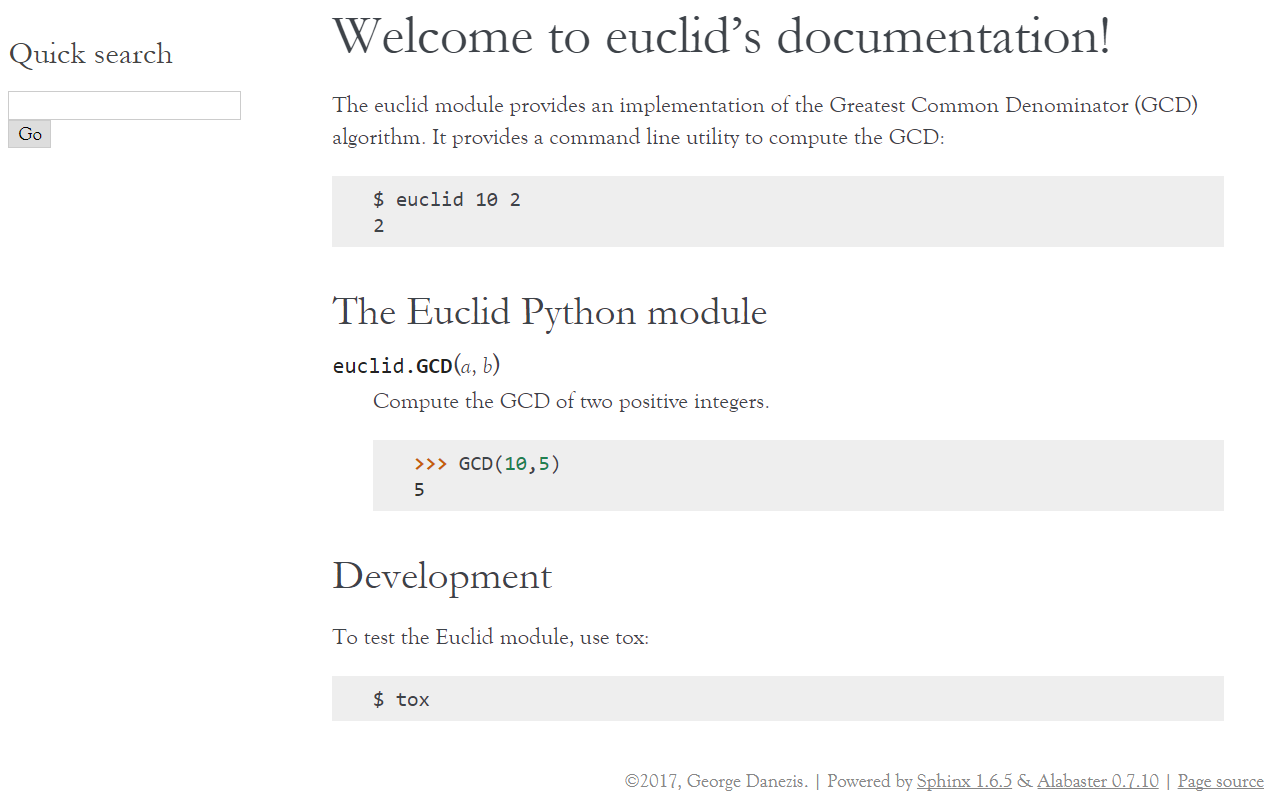
\includegraphics[scale=0.5]{assets/docs}
\end{center}

\end{frame}



\begin{frame}

\frametitle{Remember: Done Done!}

The quality installation, packaging, documentation, distinguishes the great engineer:
\begin{itemize}
  \item Always fold your projects into one or more modules.
  \item Provide packaging facilities through \texttt{setup} scrips.
  \item Allow installation through \texttt{pip}.
  \item Test in multiple environments using \texttt{tox}.
  \item Include \texttt{coverage} checking routinely in your QA process.
  \item Test packaging and deployment.
  \item Include and test documentation with \texttt{Sphinx}
  \item Upload into \texttt{pypi}, \texttt{travis}, \texttt{coveralls} and \texttt{readthedocs} \ldots
\end{itemize}

\vspace{3mm}
When learning other languages find the equivalent facilities.

\end{frame}



\bibliographystyle{alpha}
\nobibliography{references}

\end{document}
